% Beamer template generated from the handwritten outline.
% Add your final image files next to this .tex file, using the filenames in each placeholder.
% If an image file is missing, a labelled placeholder box is shown instead.

\documentclass[aspectratio=169]{beamer}

% Oxford Maths theming, with a fallback so the file still compiles elsewhere.
\IfFileExists{beamerthemeoxfordmaths.sty}{%
  \usetheme{oxfordmaths}%
}{%
  \usetheme{Madrid}%
  \usecolortheme{default}%
}

\usepackage{amsmath,amssymb,mathtools}
\usepackage{graphicx}
\usepackage{tikz}
\usepackage{appendixnumberbeamer}
\usepackage{booktabs}
\usepackage{ragged2e}
\usepackage{xcolor}
\usepackage[most]{tcolorbox}
\usetikzlibrary{positioning, arrows.meta, shapes.geometric, decorations.pathreplacing, calc}

% Hide Beamer's navigation icons in the footer.
\setbeamertemplate{navigation symbols}{}

% Colours copied from the reference style file.
\definecolor{softblue}{RGB}{232,238,246}
\definecolor{softpink}{RGB}{252,232,242}
\definecolor{softyellow}{RGB}{255,248,220}
\definecolor{softpurple}{RGB}{242,232,245}
\definecolor{softgreen}{RGB}{232,245,236}
\definecolor{softorange}{RGB}{255,239,222}
\definecolor{darkblue}{RGB}{0,33,71}
\definecolor{darkpink}{RGB}{155,65,105}
\definecolor{darkyellow}{RGB}{150,110,20}
\definecolor{darkpurple}{RGB}{95,55,120}
\definecolor{darkgreen}{RGB}{40,120,75}
\definecolor{darkorange}{RGB}{180,95,20}
\definecolor{RoadBlue}{RGB}{0,0,205}
\definecolor{RoadGreen}{RGB}{0,100,0}
\definecolor{RoadRed}{RGB}{200,0,0}
\definecolor{OxfordBlue}{RGB}{0,33,71}
\definecolor{SoftBlue}{RGB}{232,241,250}
\definecolor{SoftGreen}{RGB}{239,248,241}
\definecolor{SoftGold}{RGB}{255,247,230}
\definecolor{SoftRed}{RGB}{252,238,238}
\definecolor{TextGrey}{RGB}{84,92,105}
\definecolor{TimelineDone}{RGB}{76,160,88}
\definecolor{TimelineTheory}{RGB}{210,77,73}
\definecolor{TimelineModel}{RGB}{54,127,199}
\definecolor{TimelineVerify}{RGB}{235,154,52}
\definecolor{TimelineWrite}{RGB}{119,90,178}

% User TikZ colours.
\definecolor{meshOrange}{RGB}{238,145,0}
\definecolor{cellGreen}{RGB}{135,220,20}
\definecolor{eigenPurple}{RGB}{155,0,190}
\definecolor{axisGray}{RGB}{75,85,85}

\newtcolorbox{specbox}[2]{
    enhanced,
    colback=#1!5,
    colframe=#1!75!black,
    coltitle=white,
    colbacktitle=#1!75!black,
    title=#2,
    arc=2mm,
    boxrule=0pt,
    left=2mm,
    right=2mm,
    top=1mm,
    bottom=1mm,
    fonttitle=\bfseries
}

% Figure placeholder. Replace the filename in the third argument with your image.
% Usage: \placeholderfigure[width]{height}{filename}{label text}
\newcommand{\placeholderfigure}[4][0.80\linewidth]{%
\begin{figure}
\centering
\IfFileExists{#3}{%
  \includegraphics[width=#1]{#3}%
}{%
  \fbox{\begin{minipage}[c][#2][c]{#1}
    \centering
    \vspace{0.3em}
    {\large #4}\par\vspace{0.4em}
    {\scriptsize Replace with \texttt{\detokenize{#3}}}
  \end{minipage}}%
}%
\end{figure}%
}

% Image placeholder without a nested figure environment.
% Usage: \placeholdergraphic[width]{height}{filename}{label text}
\newcommand{\placeholdergraphic}[4][0.80\linewidth]{%
\IfFileExists{#3}{%
  \includegraphics[width=#1]{#3}%
}{%
  \fbox{\begin{minipage}[c][#2][c]{#1}
    \centering
    \vspace{0.3em}
    {\large #4}\par\vspace{0.4em}
    {\scriptsize Replace with \texttt{\detokenize{#3}}}
  \end{minipage}}%
}%
}

\newcommand{\eps}{\varepsilon}
\newcommand{\Sp}{\operatorname{Sp}}
\newcommand{\Grid}{\operatorname{Grid}}
\newcommand{\dist}{\operatorname{dist}}
\newcommand{\rot}{\operatorname{rot}}
\newcommand{\defeq}{\coloneqq}

% \title[Efficient Spectral Computations]{An Update on Our Project: Efficient Algorithms for Infinite-Dimensional Spectral Computations}
% \author{Maggie McCarthy, Patrick Farrell, Umberto Zerbinat}
% \institute{Mathematical Institute\\University of Oxford}
% \date{\today}

\title[Efficient Spectral Computations]
{An Update on Our Project: Efficient Algorithms for Infinite-Dimensional Spectral Computations}
\author[McCarthy, Farrell, Zerbinati]
{Maggie McCarthy, Patrick Farrell, Umberto Zerbinati}
% \institute{Mathematical Institute\\University of Oxford}
\date{\today}

\begin{document}

% -----------------------------------------------------------------------------
\begin{frame}[plain]
  \titlepage
\end{frame}

% -----------------------------------------------------------------------------
\begin{frame}{Motivation}
\begin{overlayarea}{\textwidth}{\textheight}

\begin{itemize}
    \item<1-> Colbrook's algorithm avoids the pitfalls of the usual ``discretize and solve'' approach.
    \item<2-> However, for coarse discretizations of the folded problems, the computed lower bound on the distance to the spectrum may not be tight.
\end{itemize}

\vspace{0.15cm}

\begin{columns}[T,onlytextwidth]
\begin{column}{0.48\textwidth}
    \only<3->{%
        \centering
        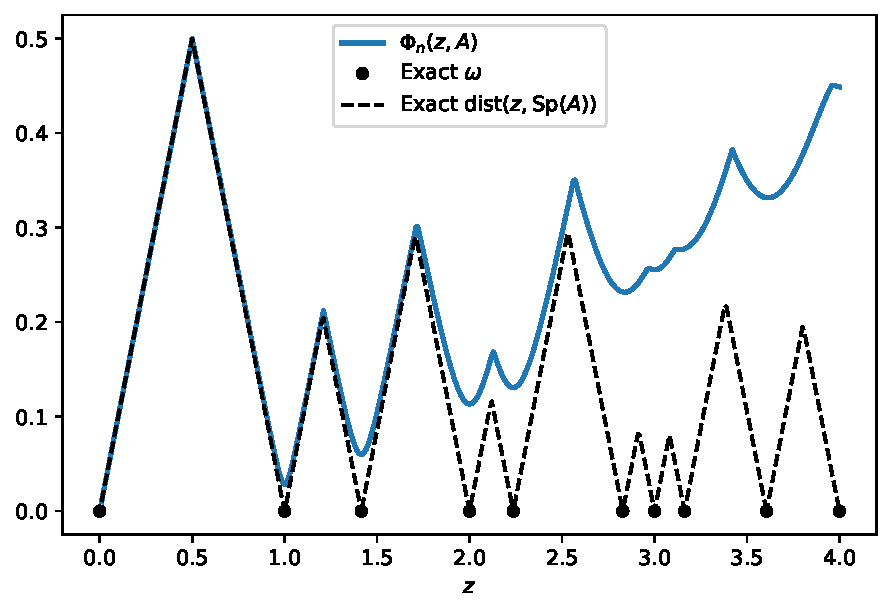
\includegraphics[width=0.90\linewidth]{dist_plot_N=32 (2).pdf}\par
        \small $N=32$
    }
\end{column}
\begin{column}{0.48\textwidth}
    \only<4->{%
        \centering
        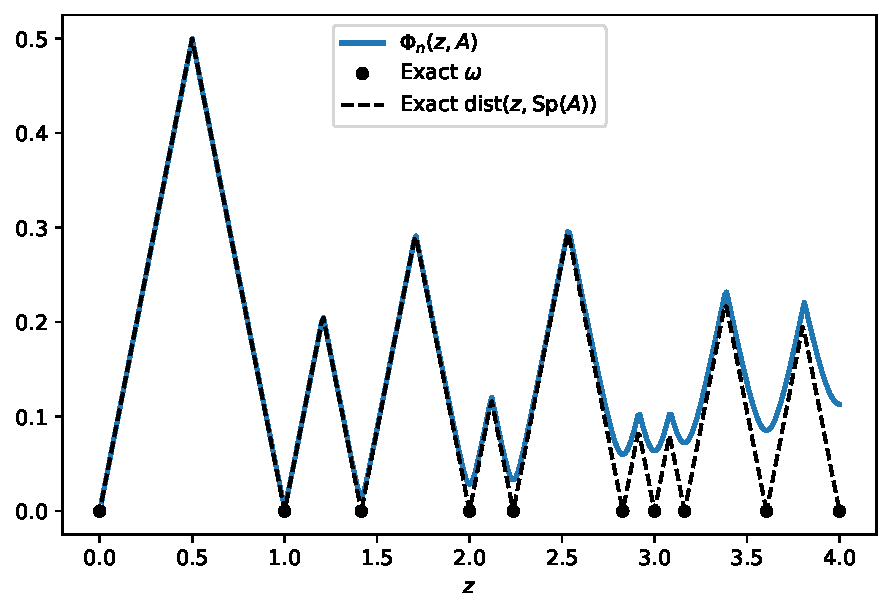
\includegraphics[width=0.90\linewidth]{dist_plot_N=128 (3).pdf}\par
        \small $N=128$
    }
\end{column}
\end{columns}

\end{overlayarea}
\end{frame}

% -----------------------------------------------------------------------------
\begin{frame}{First Idea: Apply Adaptivity to the Eigenproblems}
\begin{overlayarea}{\textwidth}{0.87\textheight}

\begin{itemize}
    \item<1-> We discretize the Rayleigh quotients defining $\gamma(z,A)$ and obtain generalized eigenproblems.
    \item<2-> We compute the smallest eigenvalues to form $\Phi_n(z,A)$.
\end{itemize}

\vspace{0.45cm}

\only<3->{
\begin{specbox}{blue}{Use an eigenvalue error estimate in two ways}
We want to improve $\Phi_n(z,A)$ using an error estimate for the auxiliary eigenvalue computations.

\vspace{0.15cm}

\begin{enumerate}
    \item<4-> Correct the eigenvalues, thereby correcting $\Phi_n(z,A)$.
    \item<5-> Drive adaptive mesh refinement for the eigensolves.
\end{enumerate}
\end{specbox}
}

\end{overlayarea}
\end{frame}

% -----------------------------------------------------------------------------
\begin{frame}{DWR for Symmetric Eigenproblems}
\begin{overlayarea}{\textwidth}{0.87\textheight}

\begin{itemize}
    \item<1-> Let $A: V \to V^*$ be self-adjoint, as is the case for the folded operator.
    \item<2-> Consider the symmetric generalized eigenproblem
    \[
        A u = \lambda M u .
    \]
    \item<3-> Define sesquilinear forms
    \[
        a(u,v)=\langle A u,v\rangle,
        \qquad
        m(u,v)=\langle M u,v\rangle .
    \]
\end{itemize}

\vspace{-0.25cm}

\begin{columns}[T,onlytextwidth]
\begin{column}{0.49\textwidth}
\only<4->{
\begin{specbox}{green!45!black}{Continuous problem}
Find $(u,\lambda)\in V\times\mathbb{C}$ such that
\[
    a(u,v)=\lambda m(u,v)\quad \forall v\in V .
\]
\end{specbox}
}
\end{column}
\begin{column}{0.49\textwidth}
\only<5->{
\begin{specbox}{purple}{Discrete problem}
Find $(u_h,\lambda_h)\in V_h\times\mathbb{C}$ such that
\[
    a(u_h,v_h)=\lambda_h m(u_h,v_h)\quad \forall v_h\in V_h .
\]
\end{specbox}
}
\end{column}
\end{columns}

\end{overlayarea}
\end{frame}

% -----------------------------------------------------------------------------
\begin{frame}{DWR for Symmetric Eigenproblems}
\begin{overlayarea}{\textwidth}{0.87\textheight}

\begin{itemize}
    \item<1-> DWR gives an error representation for the eigenvalue error.
    \item<2-> The same estimate can be used both for correction and for driving mesh refinement.
\end{itemize}

\vspace{0.15cm}

\only<3->{
\begin{specbox}{green!45!black}{DWR Method for a Symmetric Eigenproblem}
Consider an eigenpair $\{u_h,\lambda_h\}\in V_h\times\mathbb{C}$ solving the Galerkin eigenproblem. Define the primal eigenvalue residual
\[
    \rho(u_h,\lambda_h)(\cdot) \defeq a(u_h,\cdot)-\lambda_h m(u_h,\cdot).
\]
Then, for arbitrary $\varphi_h\in V_h$,
\[
    (\lambda-\lambda_h)(1-\xi_h)
    =
    \rho(u_h,\lambda_h)(u-\varphi_h),
    \qquad
    \xi_h=\frac12 m(u-u_h,u-u_h).
\]
\end{specbox}
}

\end{overlayarea}
\end{frame}

% -----------------------------------------------------------------------------
\begin{frame}{Application to Maxwell}
\begin{overlayarea}{\textwidth}{0.87\textheight}

\begin{itemize}
    \item Start on an unstructured mesh with $\operatorname{maxh}=\pi/32$.
    \item Apply five fixed levels of adaptivity for each $z$.
\end{itemize}

\vspace{0.15cm}

\begin{center}
    \only<1>{%
        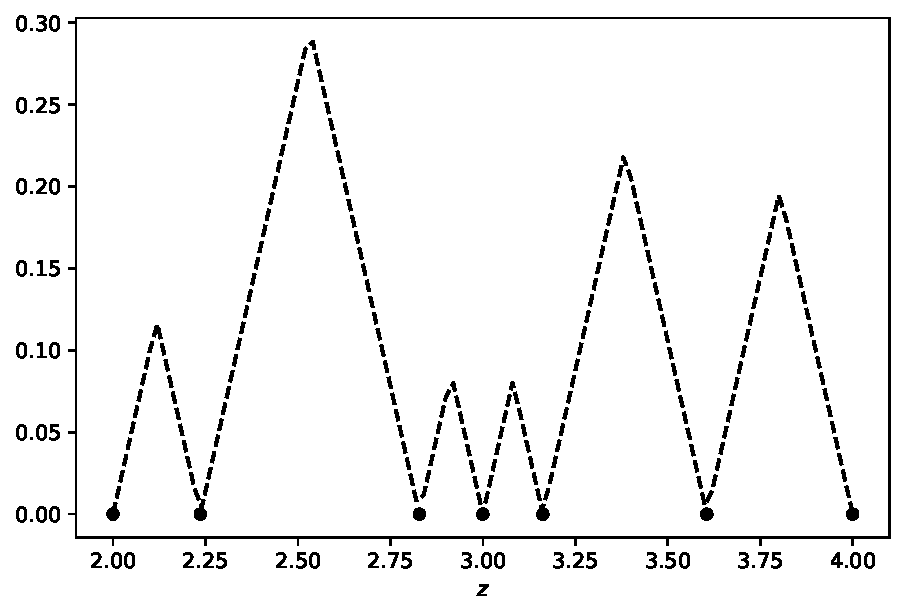
\includegraphics[width=0.5\linewidth]{plot1_N=32.pdf}
    }
    \only<2>{%
        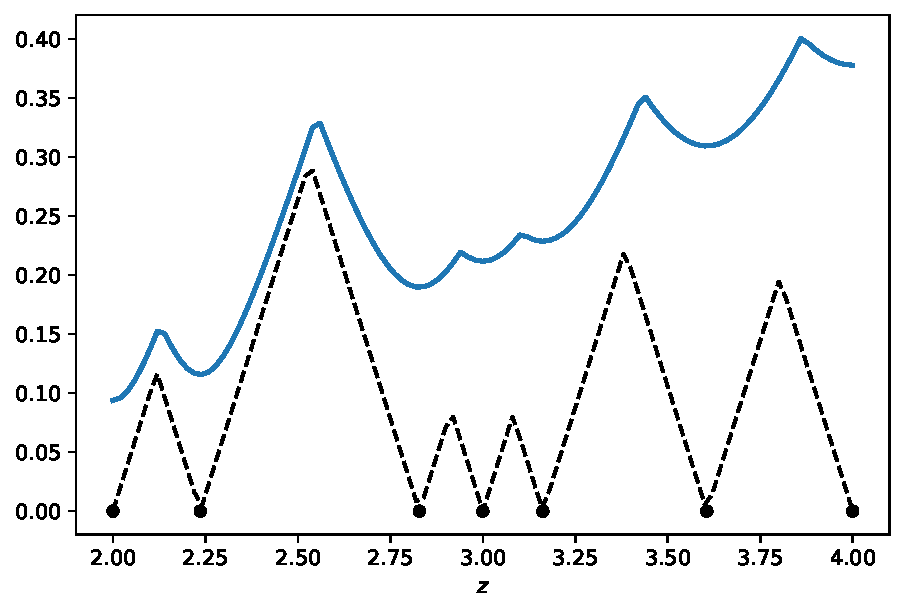
\includegraphics[width=0.5\linewidth]{plot2_N=32.pdf}
    }
    \only<3>{%
        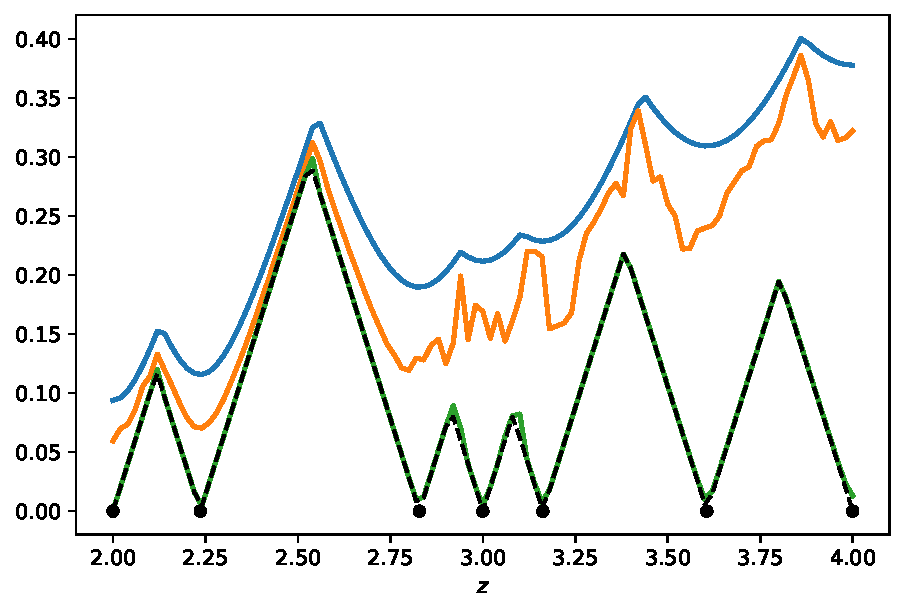
\includegraphics[width=0.5\linewidth]{plot3_N=32.pdf}
    }
\end{center}

\end{overlayarea}
\end{frame}
% -----------------------------------------------------------------------------
\begin{frame}{Some Adapted Meshes}

\begin{columns}[T,onlytextwidth]
\begin{column}{0.48\textwidth}
\centering
\placeholdergraphic[0.95\linewidth]{4.2cm}{adapted_mesh_z1.pdf}{Adapted mesh for $z=z_1$}

\vspace{0.15cm}
{\footnotesize (a) Adapted mesh for $z=z_1$}
\end{column}
\begin{column}{0.48\textwidth}
\centering
\placeholdergraphic[0.95\linewidth]{4.2cm}{adapted_mesh_z2.pdf}{Adapted mesh for $z=z_2$}

\vspace{0.15cm}
{\footnotesize (b) Adapted mesh for $z=z_2$}
\end{column}
\end{columns}

\end{frame}

% -----------------------------------------------------------------------------
\begin{frame}{Next Idea: Inner and Outer Refinement}
\begin{overlayarea}{\textwidth}{0.87\textheight}

\begin{itemize}
    \item<1-> We want accurate and efficient pseudospectral pictures in the complex plane.
\end{itemize}

\vspace{0.55cm}

\only<2->{To achieve this, we couple two refinement processes:}

\vspace{0.35cm}

\begin{enumerate}
    \item<3-> {\Large\textbf{Complex-plane refinement}}\\[0.12cm]
    \hspace*{0.8cm}Refine triangles near the estimated $\eps$-contour.

    \vspace{0.45cm}

    \item<4-> {\Large\textbf{Eigenproblem refinement}}\\[0.12cm]
    \hspace*{0.8cm}Refine the finite element meshes used for the folded eigensolves.
\end{enumerate}

\end{overlayarea}
\end{frame}

% -----------------------------------------------------------------------------
\begin{frame}{Inner Refinement}
\begin{overlayarea}{\textwidth}{0.87\textheight}

\begin{itemize}
    \item<1-> DWR yields an error estimate for each auxiliary eigenproblem:
\end{itemize}

\only<1->{
\[
    \eta^{(1)}(z) \approx \lambda^{(1)}(z)-\lambda_h^{(1)}(z),
    \qquad
    \eta^{(2)}(z) \approx \lambda^{(2)}(z)-\lambda_h^{(2)}(z).
\]
}

\vspace{0.25cm}

\begin{itemize}
    \item<2-> Using the definitions of $\gamma(z,A)$ and $\Phi_n(z,A)$, we obtain a computable error bound for $\Phi_n(z,A)$:
\end{itemize}

\only<2->{
\begin{specbox}{green!45!black}{Inner error bound}
\[
    \left|\gamma(z,A)-\Phi_n(z,A)\right|
    \leq
    \sqrt{\left|\eta^{(1)}(z)\right|}
    +
    \sqrt{\left|\eta^{(2)}(z)\right|} .
\]
\end{specbox}
}

\end{overlayarea}
\end{frame}

% -----------------------------------------------------------------------------
\begin{frame}{Outer Refinement Criteria}
\begin{overlayarea}{\textwidth}{0.87\textheight}

\begin{columns}[T,onlytextwidth]
\begin{column}{0.47\textwidth}
\begin{itemize}
    \item<1-> Given the desired $\eps$ for the pseudospectrum, triangulate the complex plane.

    \vspace{0.25cm}

    \item<2-> Index the cells by $K$, with barycentre $z_K$ and diameter $h_K$.

    \vspace{0.25cm}

    \item<3-> Define the grid of test points by
    \[
        \Grid = \{z_K : K\in\mathcal{T}_k\}.
    \]
\end{itemize}
\end{column}
\begin{column}{0.50\textwidth}
\centering
\begin{tikzpicture}[
    scale=1.15,
    axis/.style={
        axisGray,
        very thick,
        -{Latex[length=3mm,width=2.5mm]}
    },
    mesh/.style={
        gray!90,
        thick,
        dashed
    },
    selected cell/.style={
        cellGreen!90!black,
        very thick
    },
    barycentre/.style={
        circle,
        fill=eigenPurple,
        inner sep=2.1pt
    }
]

% Axes
\draw[axis] (-1.55,0) -- (2.35,0)
    node[right, axisGray] {$\operatorname{Re} z$};
\draw[axis] (0,-1.75) -- (0,1.95)
    node[above, axisGray] {$\operatorname{Im} z$};
\node[axisGray] at (2.25,1.45) {\Large $\mathbb{C}$};

% Triangulation
\only<1->{
\foreach \x in {-1,0,1,2}
    \draw[mesh] (\x,-1.5) -- (\x,1.5);
\foreach \y in {-1.5,-0.5,0.5,1.5}
    \draw[mesh] (-1,\y) -- (2,\y);
\foreach \x in {-1,0,1}{
    \foreach \y in {-1.5,-0.5,0.5}{
        \draw[mesh] (\x,\y) -- ++(1,1);
    }
}
\node[gray!90, font=\bfseries] at (-0.72,1.72) {$\mathcal{T}_k$};
}

% Highlighted triangular cell K
\only<2->{
\fill[cellGreen, opacity=0.22]
    (-1,-0.5) -- (0,-0.5) -- (0,0.5) -- cycle;
\draw[selected cell]
    (-1,-0.5) -- (0,-0.5) -- (0,0.5) -- cycle;
\node[cellGreen!90!black, font=\bfseries\scriptsize]
    at (-0.73,-0.38) {$K$};
\coordinate (zK) at (-0.333,-0.167);
\node[barycentre] at (zK) {};
\node[cellGreen!90!black, font=\bfseries\scriptsize, below=2pt]
    at (zK) {$z_K$};
}

% Barycentres of all triangles
\only<3->{
\foreach \x in {-1,0,1}{
    \foreach \y in {-1.5,-0.5,0.5}{
        \node[barycentre] at ({\x+2/3},{\y+1/3}) {};
        \node[barycentre] at ({\x+1/3},{\y+2/3}) {};
    }
}
\coordinate (zK) at (-0.333,-0.167);
\node[barycentre] at (zK) {};
\node[cellGreen!90!black, font=\bfseries\scriptsize, below=2pt]
    at (zK) {$z_K$};
\node[eigenPurple, font=\bfseries]
    at (1.15,1.72) {Grid};
}
\end{tikzpicture}
\end{column}
\end{columns}

\end{overlayarea}
\end{frame}

% -----------------------------------------------------------------------------
\begin{frame}{Outer Refinement Criteria: Error on a Cell}

For any $w\in K$, using that $\gamma(\cdot,A)$ is $1$-Lipschitz,
\[
\begin{aligned}
    \left|\gamma(w,A)-\Phi_n(z_K,A)\right|
    &\leq |w-z_K| + \left|\gamma(z_K,A)-\Phi_n(z_K,A)\right| \\
    &\leq h_K
    + \sqrt{\left|\eta^{(1)}(z_K)\right|}
    + \sqrt{\left|\eta^{(2)}(z_K)\right|} \\
    &:= R_K .
\end{aligned}
\]

\vspace{0.3cm}

Rearranging gives
\begin{specbox}{green!45!black}{For all $w\in K$}
\[
    \Phi_n(z_K,A)-R_K
    \leq
    \gamma(w,A)
    \leq
    \Phi_n(z_K,A)+R_K .
\]
\end{specbox}

\end{frame}

% -----------------------------------------------------------------------------
\begin{frame}{Outer Refinement}
\begin{overlayarea}{\textwidth}{0.87\textheight}

From the enclosure
\[
    \Phi_n(z_K,A)-R_K
    \leq
    \gamma(w,A)
    \leq
    \Phi_n(z_K,A)+R_K,
    \qquad w\in K,
\]
we classify each triangle as follows.

\vspace{0.2cm}

\begin{enumerate}
    \item<1-> If $\Phi_n(z_K,A)+R_K<\eps$, mark $K$ as inside the $\eps$-pseudospectrum.
    \item<2-> If $\Phi_n(z_K,A)-R_K>\eps$, mark $K$ as outside the $\eps$-pseudospectrum.
    \item<3-> Otherwise, refine $K$ by connecting the midpoints of its edges.
\end{enumerate}

\vspace{0.05cm}

\only<3->{
\begin{center}
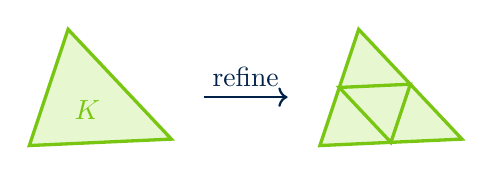
\begin{tikzpicture}[scale=0.82]
    \draw[fill=cellGreen!20, draw=cellGreen!90!black, very thick] (0,0) -- (2.2,0.1) -- (0.6,1.8) -- cycle;
    \node[cellGreen!90!black,font=\bfseries] at (0.9,0.55) {$K$};
    \draw[->, thick, OxfordBlue] (2.7,0.75) -- (4.0,0.75) node[midway,above]{refine};
    \coordinate (A) at (4.5,0); \coordinate (B) at (6.7,0.1); \coordinate (C) at (5.1,1.8);
    \coordinate (MAB) at ($(A)!0.5!(B)$); \coordinate (MBC) at ($(B)!0.5!(C)$); \coordinate (MCA) at ($(C)!0.5!(A)$);
    \draw[draw=cellGreen!90!black, very thick, fill=cellGreen!20] (A)--(B)--(C)--cycle;
    \draw[cellGreen!90!black, very thick] (MAB)--(MBC)--(MCA)--cycle;
\end{tikzpicture}
\end{center}
}

\end{overlayarea}
\end{frame}

% -----------------------------------------------------------------------------
\begin{frame}{The Coupling}
\begin{overlayarea}{\textwidth}{0.87\textheight}

\begin{enumerate}
    \item<1-> Iterate over the barycentres $z_K$.
    \item<2-> Solve the two folded eigenproblems until
    \[
        \left|\eta^{(1)}(z_K)\right| \leq \frac{h_K^2}{2},
        \qquad
        \left|\eta^{(2)}(z_K)\right| \leq \frac{h_K^2}{2},
    \]
    or until the maximum degree-of-freedom limit is reached.
    \item<3-> Check the outer refinement criteria.
    \item<4-> Repeat the process on the new set of triangles produced by outer refinement.
    \item<5-> Stop once remaining triangles reach the diameter tolerance; these are marked as contour triangles.
\end{enumerate}

\end{overlayarea}
\end{frame}

% -----------------------------------------------------------------------------
\begin{frame}{Example: Dirac Poisson}

Let
\[
    U=\begin{pmatrix}u\\ \sigma\end{pmatrix},
    \qquad
    AU=\begin{pmatrix}-i\sigma'\\ -iu'\end{pmatrix},
    \qquad
    D(A)=H_0^1(0,\pi)\times H^1(0,\pi).
\]

\vspace{0.15cm}

To relate this back to the Poisson eigenproblem, consider $AU=\lambda U$. Solving for $\sigma$ in the second equation and substituting into the first gives
\[
    -u''=\lambda^2 u .
\]

\vspace{0.1cm}

Thus the eigenvalues are
\[
    \lambda=0,\quad \lambda=\pm n,\qquad n=1,2,\ldots .
\]

\end{frame}

% -----------------------------------------------------------------------------
\begin{frame}{Results: Dirac Poisson, $\varepsilon = 0.2,$ diameter tolerance $0.01.$}
\begin{overlayarea}{\textwidth}{0.87\textheight}

\begin{center}
    \only<1>{%
        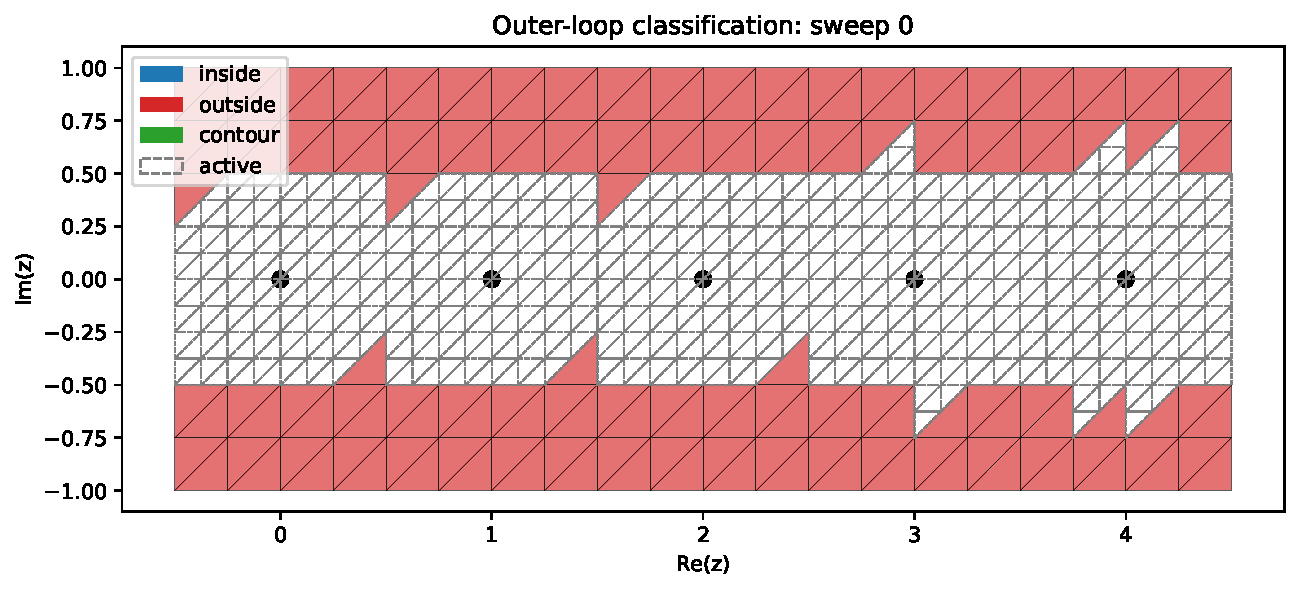
\includegraphics[
            width=0.95\textwidth,
            height=0.78\textheight,
            keepaspectratio
        ]{sweep0 (1).pdf}
    }
    \only<2>{%
        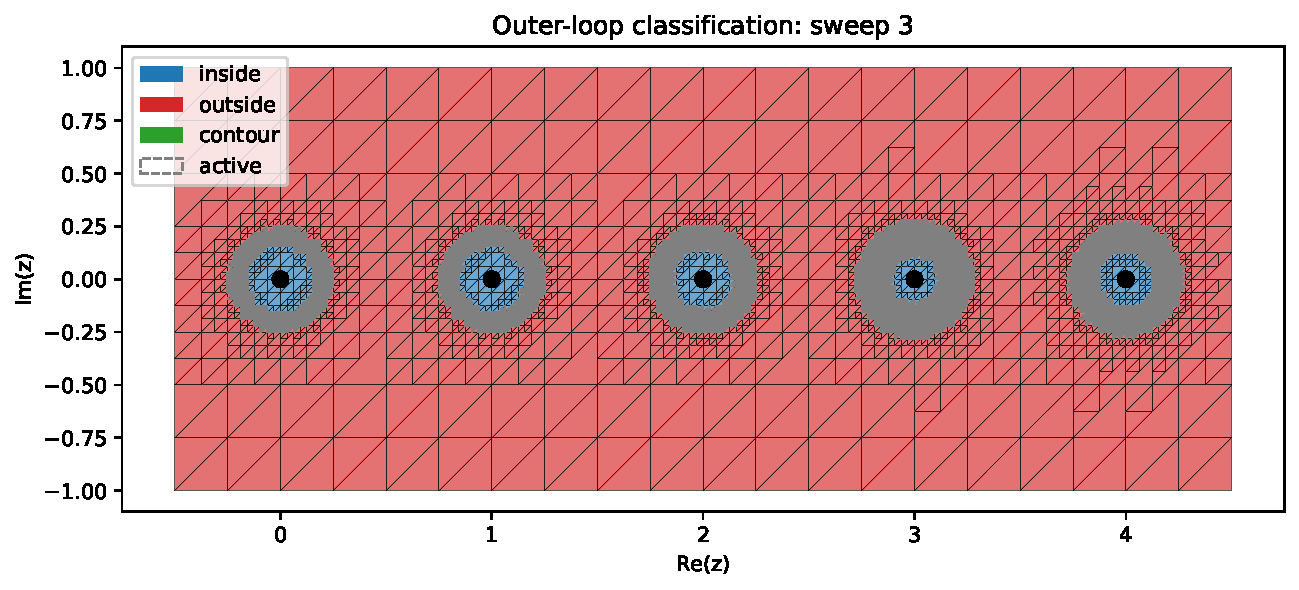
\includegraphics[
            width=0.95\textwidth,
            height=0.78\textheight,
            keepaspectratio
        ]{sweep3 (1).pdf}
    }
    \only<3>{%
        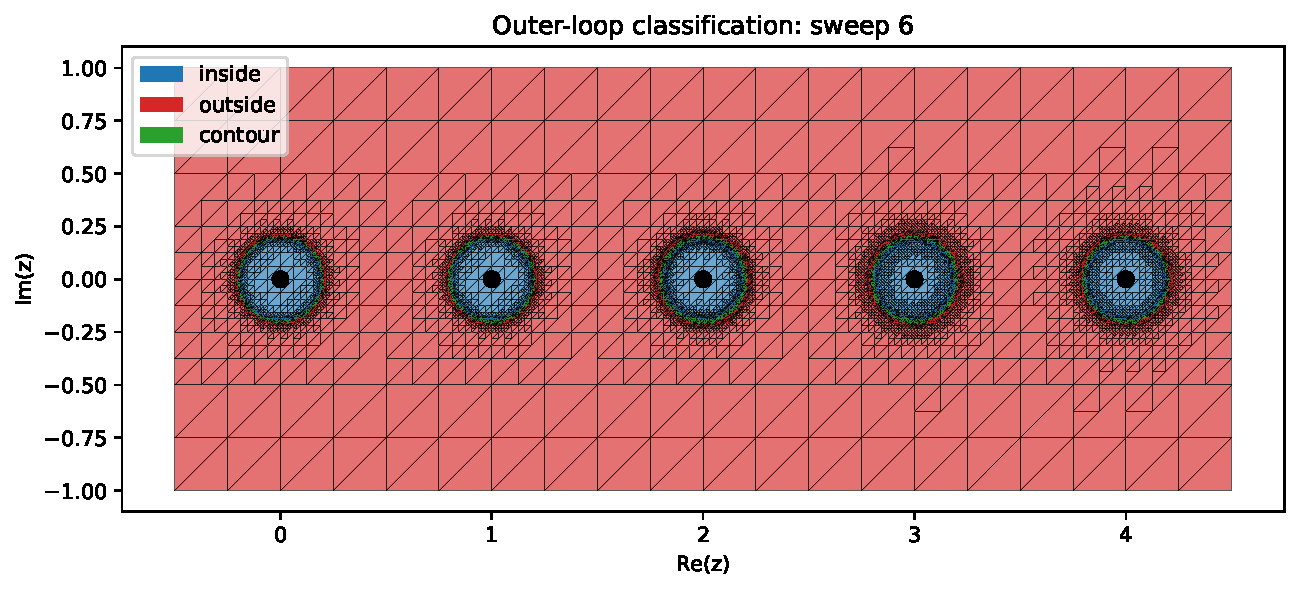
\includegraphics[
            width=0.95\textwidth,
            height=0.78\textheight,
            keepaspectratio
        ]{sweep6 (1).pdf}
    }
\end{center}
\end{overlayarea}
\end{frame}

% -----------------------------------------------------------------------------
\begin{frame}{More Results: Zoom In At Sweep 6}

\begin{center}
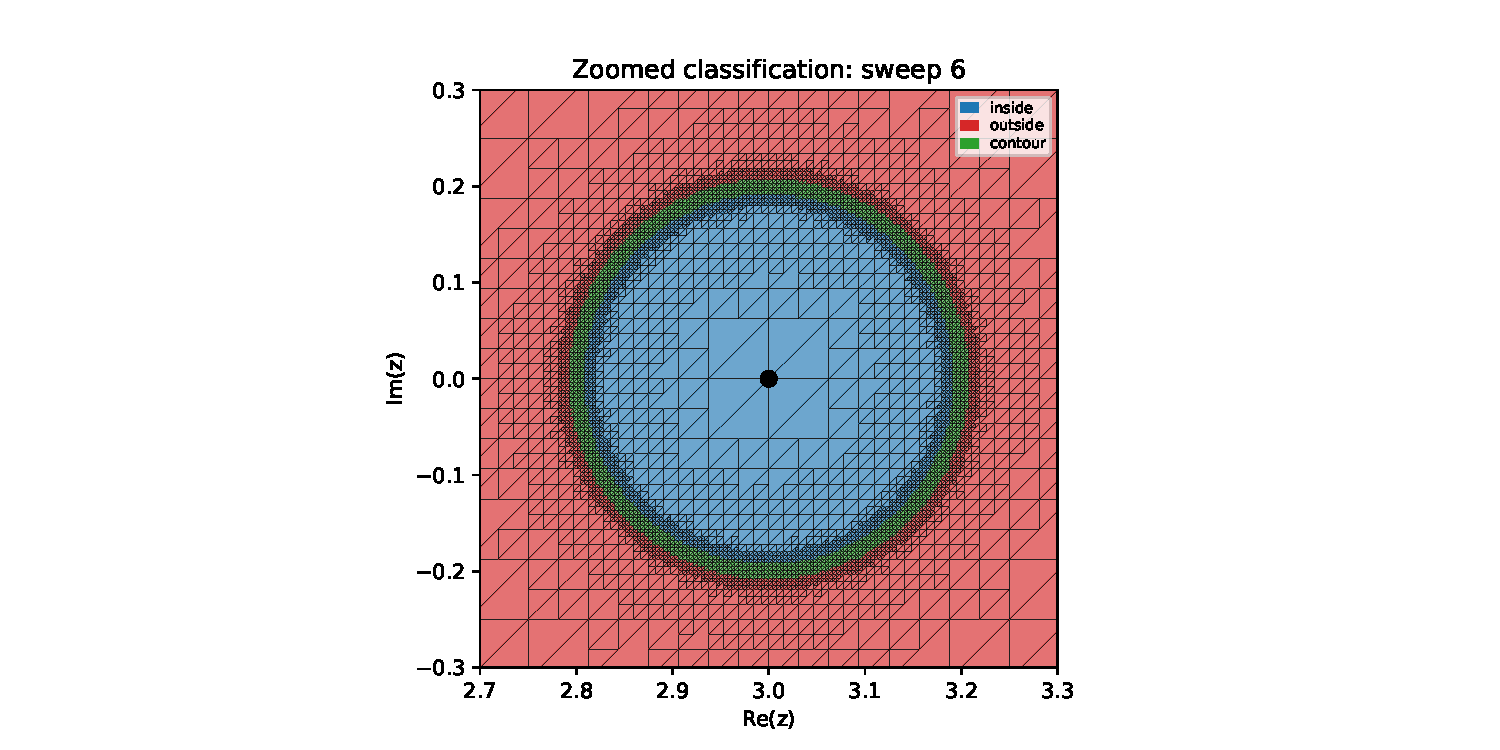
\includegraphics[
            width=0.95\textwidth,
            height=0.95\textheight,
            keepaspectratio
        ]{zoomin (1).pdf}
\end{center}

\end{frame}


% -----------------------------------------------------------------------------
\begin{frame}{Example: Maxwell}

On $U=(0,\pi)^2$, find $\omega\in\mathbb{R}\setminus\{0\}$ and nonzero
$(E,H)\in H_0(\rot;U)\times H(\rot;U)$ such that
\[
    \rot E = i\omega H,
    \qquad
    \rot H = -i\omega E,
    \qquad
    E\cdot t =0 \text{ on }\partial U .
\]

\vspace{0.15cm}

The operator we fold is
\[
    M_{2D}(E,H)=\bigl(i\rot H,\,-i\rot E\bigr),
    \qquad
    D(M_{2D})=H_0(\rot;U)\times H(\rot;U).
\]

\vspace{0.15cm}

On $(0, \pi)^2$, the eigenvalues are
\[
    \omega=0,
    \qquad
    \omega=\pm\sqrt{m^2+n^2},
    \qquad m,n\in\mathbb{N}_0 .
\]

\end{frame}

% -----------------------------------------------------------------------------
\begin{frame}{Results: Maxwell, $\varepsilon = 0.2,$ diameter tolerance $0.02.$}
\begin{overlayarea}{\textwidth}{0.87\textheight}

\begin{center}
    \only<1>{%
        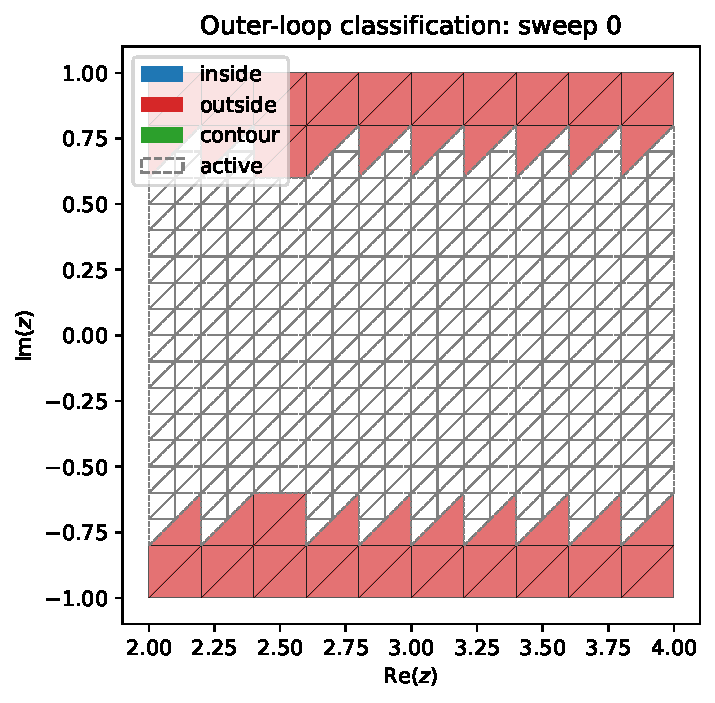
\includegraphics[
            width=0.95\textwidth,
            height=0.78\textheight,
            keepaspectratio
        ]{sweep_000 (1).pdf}
    }
    \only<2>{%
        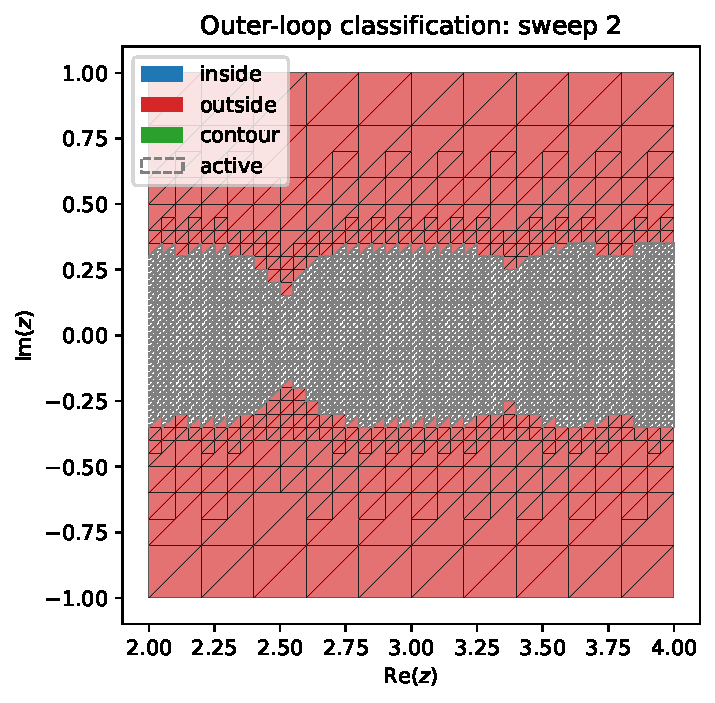
\includegraphics[
            width=0.95\textwidth,
            height=0.78\textheight,
            keepaspectratio
        ]{sweep_002 (1).pdf}
    }
    \only<3>{%
        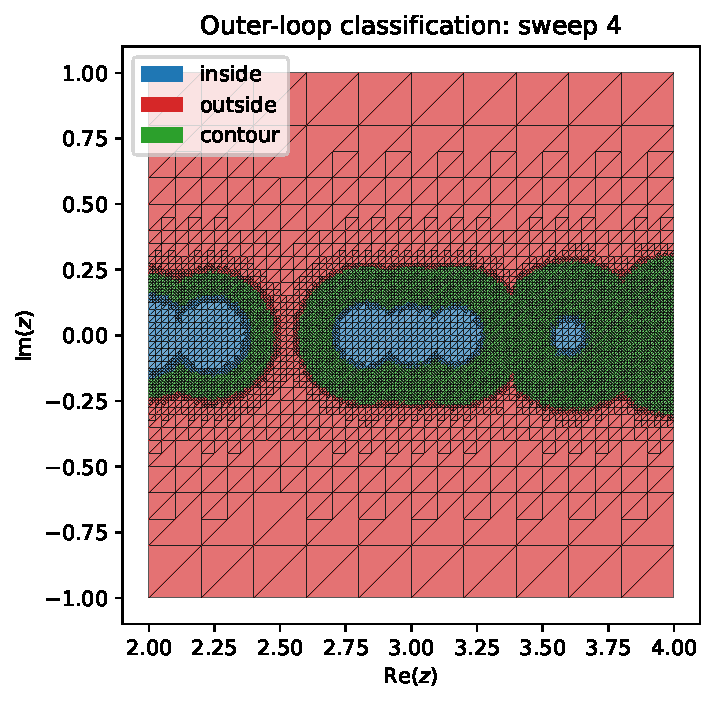
\includegraphics[
            width=0.95\textwidth,
            height=0.78\textheight,
            keepaspectratio
        ]{sweep_004 (1).pdf}
    }
\end{center}
\end{overlayarea}
\end{frame}


% -----------------------------------------------------------------------------
\begin{frame}{To Be Continued}

\begin{itemize}
    \item Further experimentation with inner and outer coupling.

    \vspace{0.45cm}

    \item Apply the approach to one-dimensional advection--diffusion.

    \vspace{0.45cm}

    \item Several new research directions are emerging:
    \begin{itemize}
        \item expanding DWR to handle general spectral values;
        \item multilevel methods exploiting the hierarchy of DWR-refined meshes;
        \item sharper coupling rules between inner and outer refinement.
    \end{itemize}
\end{itemize}

\end{frame}

\end{document}
